
\documentclass[10pt]{article}
\usepackage[utf8]{inputenc}
\usepackage{kotex}
\usepackage{graphicx}
\usepackage{subfigure}
\usepackage{titling}
\setlength{\droptitle}{-2cm}
\usepackage{array}
\usepackage{amssymb}
\usepackage{amsmath}
\usepackage{siunitx} 
\usepackage{enumerate} 
\usepackage{pgfplots}
\usepackage{pgfplotstable}
\usepackage{tikz,pgfplots}
\usepackage{wasysym}
\usepackage{geometry}
\usepackage{authblk}
\usepackage{kotex}
\usepackage{bibunits}
\usepackage{tabularx}
\usepackage{hyperref}
\usepackage{pythonhighlight}
\usepackage{bbm}

\geometry{
    a4paper,
    total={170mm,257mm},
    left=20mm,
    top=20mm,
}

\title{\textbf{Mathematical Foundation of DNN : HW 1}}
\author{Jeong Min Lee}

\begin{document}
\maketitle

\section*{1}
\begin{figure}[!h]
    \begin{center}
        \subfigure[]{
            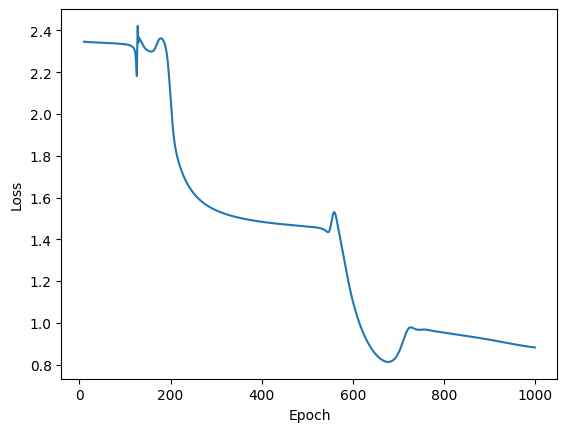
\includegraphics[scale = 0.5]{../hw3/fig/fig1_1.png}
        }
        \subfigure[]{
            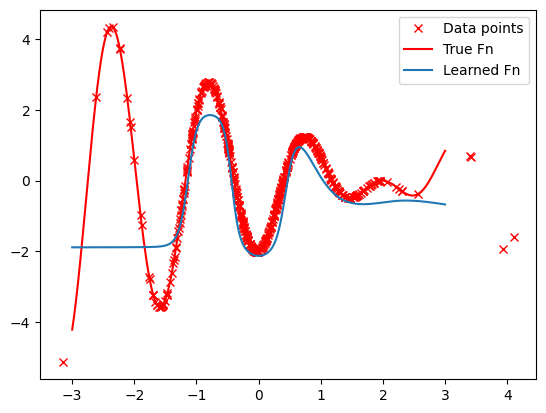
\includegraphics[scale = 0.5]{../hw3/fig/fig1_2.png}
        }
    \end{center}
    \caption{(a) The loss of the training for each epoch. (b) The result of training.}
    \label{fig1}
\end{figure}
As figure \ref{fig1} depicts, the training was success, since the training loss was decreasing. However, this is not sufficient. 
In figure \ref{fig1} (b) says, the learned function cannot fit the true function, well, focusing on the edge of the function. 
Such insufficient performance can be verified via the test dataset. In test dataset, the test loss was $1.2830710411071777$ and the accuracy was $0.5196078431372549$, which is not enough to say that our model approximate true function well. 

\section*{2}
\begin{figure}[!h]
    \begin{center}
        \subfigure[]{
            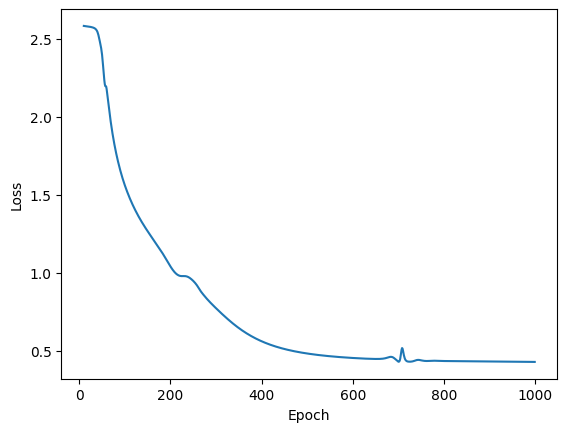
\includegraphics[scale = 0.5]{../hw3/fig/fig2_1.png}
        }
        \subfigure[]{
            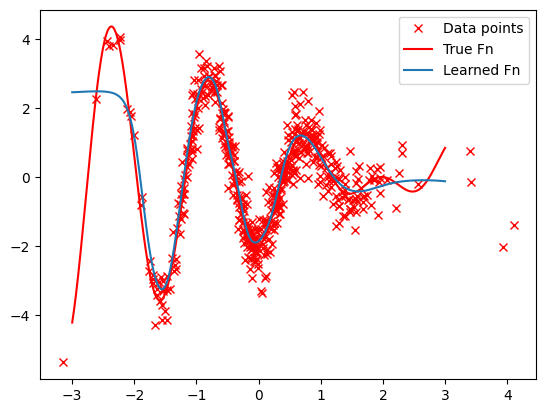
\includegraphics[scale = 0.5]{../hw3/fig/fig2_2.png}
        }
    \end{center}
    \caption{(a) The loss of the training for each epoch. (b) The result of training.}
    \label{fig2}
\end{figure}
By adding the gaussian noise in label of train dataset, as figure \ref{fig2} describes, the overall performance of model increases.
Furthermore, the test loss was $0.15671254694461823$ and accuracy was $0.9313725490196079$, which is much outperform the model trained in the dataset without the noise. 
I made some hypothesis for this weird phenomenon. In this problem, there is about 4000 parameters to be learned, while the number of the data is about 500.
This is a common setting that the model is overfitted. Overfitted model,like the model in problem 1, has really high accuracy in the train data, but the extremely low accuracy in the test data. 
Checking the figure \ref{fig1}, the model has quite good precision at the center, while not in the border. This implies that model is too focus on the interval that the data is concentrated and ignore the details. 
This problem can be solved via adding appropriate noise on the train dataset, as figure \ref{fig2} shows. In figure \ref{fig2}, the model makes an effort to focus on the center of the data and sufficiently fit the data in border. 
From these examples, we can conjecture that adding some noise or training the model with noised data(which is the common setting of DL) can keep model from being overfitted. 






\section*{3}
\subsection*{a}
\begin{align*}
    &0<-\log{\frac{\exp{f_y}}{\sum_j \exp{f_j}}}<\infty\\
    & \iff -\infty < \log(\frac{\exp{f_y}}{\sum_j \exp{f_j}})<0 \\
    & \iff 0 < \frac{\exp{f_y}}{\sum_j \exp{f_j}} <1 \\
    & \iff 0 < \mu_y(f) < 1
\end{align*}

The positivity of softmax function is trivial from $\exp(x)>0 \text{ for } \forall x \in \mathbb{R}$. 
Futhermore, since $\nexists x\in \mathbb{R} \text{ s.t. } \exp{x} =  0$, $\mu_y(f) < 1 \text{ for } \forall x \in \mathbb{R}, k>1$.
Therefore, $0<l^{CE}(f,y)<\infty$.
\subsection*{b}

\begin{align*}
    &l^{CE}(\lambda e_y,y) \rightarrow 0 \text{ as } \lambda \rightarrow \infty \\
    &\iff \frac{\exp{\lambda e_y}}{\sum_j \exp{\lambda e_y}} \rightarrow 1 \text{ as } \lambda \rightarrow \infty
\end{align*}
Let $\mu$ be the softmax function that map from $\mathbb{R}^n$ to $\mathbb{R}^n$. Then, it is enough to show the following.

\begin{equation*}
    \mu_y(\lambda e_y) \rightarrow 1 \text{ as } \lambda \rightarrow \infty
\end{equation*}

\begin{align*}
    \mu\left(\begin{bmatrix}
        0  \\ \vdots \\ \lambda \\ \vdots \\ 0 
    \end{bmatrix}\right) = \frac{1}{(k-1) + \exp{\lambda}}\begin{bmatrix}
        1  \\ \vdots \\ \exp{\lambda} \\ \vdots \\ 1 
    \end{bmatrix} \rightarrow \begin{bmatrix}
        0  \\ \vdots \\ 1 \\ \vdots \\ 0
    \end{bmatrix}
\end{align*}

Since $\mu_y(\begin{bmatrix}
    0  ,\cdots,  \lambda,  \cdots,  0
\end{bmatrix}^T) = 1$, the prove is done.

\section*{4}
Suppose $f(x_0) = f_I(x_0)$ at some point $x_0 \in \mathbb{R}$. Since $f_i$ are differentiable, they are continuous at $x_0$, which implies following.
\begin{equation}
    \forall \epsilon_1>0, \exists \delta_1>0 \text{ s.t. } |x-x_0| < \delta, |f(x) - f(x_0)| <\epsilon_1
    \label{eqn1}
\end{equation}
Equation \ref{eqn1} implies the following statemet: let $f(x)=f_i(x)$ for some $x \in [x_0-\delta,x_0+\delta]$ for some $i \in \left\{1,2,\cdots,N\right\}$. Next, from the continuity of $f$ at $x_0$, $|f(x) - f(x_0)| = |f_i(x) - f_I(x_0)| < \epsilon_1$.
The inequality above results in $f_i(x)-\epsilon_1 < f_I(x_0)$. Furthermore, from the continuity of $f_I$, for $x \in [x_0 -\delta_2, x_0 + \delta_0]$, $ |f_I(x) - f_I(x_0)| <\epsilon_2(\forall \epsilon_2>0)$, which implies $f_I(x_0) < f_I(x) + \epsilon_2$.
Then, $f_i(x)-\epsilon_1<f_I(x)+\epsilon_2$ hold for $x \in [x_0 - \delta, x_0 + \delta]$ where $\delta = \min\left\{\delta_1,\delta_2\right\}$. Since the inequality holds for arbitrarily selected $\epsilon_1, \epsilon_2$, $f_I(x) \ge f_i(x)$ for $x \in [x_0 - \delta, x_0 + \delta]$.
This implies that there is an interval that $f(x) = f_I(x)$. Now, employing the differentiability of $f_I(x)$, $f^\prime(x) = f_I^\prime(x)$ holds.

\section*{5}
\subsection*{a}
\begin{equation}
    \sigma(\sigma(z)) = \max\left\{{0,\sigma(z)}\right\} = \sigma(z) (\because \sigma(z) \ge 0 \text{ for } \forall z \in \mathbb{R})
\end{equation}

\subsection*{b}
\textbf{CLAIM : } The function whose derivative is continuous and bounded above is Lipschitz continuous.\\
\textbf{proof}\\
From Mean Value Theorem, for arbitrary $x,y \in \mathbb{R}$,(without loss of generality $x < y$)
\begin{equation*}
    \exists \zeta \in \left[x,y\right] \text{ s.t. } f(x)-f(y) = f^\prime(\zeta)(x-y)
\end{equation*}
Since we suppose that $f^\prime$ is continuous and bounded, 
\begin{equation*}
    \exists C \in \mathbb{R} \text{ s.t. } f^\prime(\zeta) \le C
\end{equation*}
Combining the equation and inequaility above, 
\begin{equation*}
    f(x) - f(y) \le C(x - y)
\end{equation*}
,which implies $f$ is Lipschitz continuous.$\blacksquare$

According to the \textbf{CLAIM} I proved above, it is enough to show that the derivative of softplus function has continuous and bounded derivative and $ReLU$ does not. 
Softplus, whose derivative is $f^\prime(x) = \frac{\exp{x}}{1+\exp{x}}$, is trivially continuous differentiable, noting that $\exp{x}$ is continuous and the denominator of $f^\prime(x)$ never be zero. 
Furthermore, the double derivative of softplus, which is $f^{\prime \prime} = \frac{\exp{x}}{(1+\exp{z})^2}$, is also continuous. Also, from the following inequailities,
\begin{equation*}
    (1+\exp{x})^2 - \exp{x} = (\exp{x})^2 + \exp{x} + 1 > 0 \text{ for } \forall x \in \mathbb{R}.
\end{equation*}
$f^{\prime \prime}$ is bounded above.
\begin{equation*}
    f^{\prime \prime} = \frac{\exp{x}}{(1+\exp{z})^2} < 1
\end{equation*}
Thus, from the \textbf{CLAIM}, softplus is Lipschitz continuous differentiable.

However, for $ReLU$ function, it has discontinuous derivative, which is discontinuous at $x = 0$. Discontinuous function never be the Lipschitz continuous, as Lipschitz continuous implies continuity of the function. Thus, the prove is done. 

\subsection*{c}
\begin{equation*}
    \rho(z) = \frac{1 - \exp{(-2z)}}{1+\exp{(-2z)}} = \frac{1}{1+\exp{(-2z)}} - \frac{\exp{(-2z)}}{1+\exp{(-2z)}} = \sigma(2z) - (1-\sigma(2z)) = 2\sigma(2z)-1
\end{equation*}
The relation above implies that tanh is sigmoid function with scaling and translation. Such transformations can be expressed by imposing some contraints on the parameters in linear regression.
To be more specific, each layer can return same output, theoratically. Consider the $j$th element of $i+1$ layer's input of both activation functions.

\begin{align*}
    \sum_k C_{i+1}^{(jk)}y_i^{(k)} + d_{i+1}^{(j)} &=\sum_k C_{i+1}^{(jk)}\tanh\left(\sum_lC_i^{(kl)}y_{i-1}^{(l)} + d_i^{(k)}\right) + d_{i+1}^{(j)}  \\
    &= \sum_k \left[ 2C_{i+1}^{(jk)}\sigma\left(2\sum_l C_i^{(kl)}y_{i-1}^{(l)} + 2d_i^{(k)}\right) - C_{i+1}^{(jk)}\right] + d_{i+1}^{(j)}
\end{align*}
I assumed that this element above can be equal in both sigmoid activated and tanh activated MLP, theoratically. To meet this end, 
\begin{equation*}
    \sum_k \left[ 2C_{i+1}^{(jk)}\sigma\left(2\sum_l C_i^{(kl)}y_{i-1}^{(l)} + 2d_i^{(k)}\right) - C_{i+1}^{(jk)}\right] + d_{i+1}^{(j)} = \sum_k A_{i+1}^{(jk)} \sigma\left(\sum_l A_i^{(kl)} y_{i-1}^{(l)} + b_i^{(k)}\right) + b_{i+1}^{(j)}
\end{equation*}
Setting $A_{i+1}^{(jk)} = 2C_{i+1}^{(jk)}, d_i^{(k)} = 2b_i^{(k)}, b_{i+1}^{(j)} = d_{i+1}^{(j)} - \sum_k C_{i+1}^{(jk)}$, the equality above hold. 
Considering the recursive relation of $b_i^{(j)}$, the following relation appears.
\begin{equation*}
    b_{i+1}^{(j)} = \sum_k C_{i+1}^{(jk)}
\end{equation*} 
This enables us to represent every weight into the element of $C$. 

\begin{align*}
    A_{i}^{(jk)} &= 2C_{i}^{(jk)} \\ b_{i}^{(j)} &= \sum_k C_{i}^{(jk)} \\ d_i^{(j)} &= 2\sum_k C_{i}^{(jk)}
\end{align*}
Imposing the contraints above, both MLP become identical for each layer. However, this is only theoratically valid, which is not practically happened.

\section*{6,7}
Let's denote the input to the $j$th $ReLU$ function at the $k$th iteration as $z^{(k)}_j = a^{(k)}_jX_i + b^{(k)}_j$. Since the $j$th $ReLU$output is dead at the initialization, we have $a^{(0)}_jX_i + b^{(0)}_j<0$ for all $i=1,\cdots,N$. Hence, the output of the $j$th ReLU is $f(z^{(0)}) = 0$.
While the training, the parameter $a^{(k)}, b^{(k)}$ are updated using gradient descent. Noting that the derivative of $ReLU$ function becomes 0 for negative input, while identity for positive input, the derivative of $ReLU$ with input $z^{(0)}_j<0$ is also zero. 
This implies that $a^{(k)}_j,b^{(k)}_j$ never be changed from their initial values and as a result, $z^{(k)}_j = a^{(k)}_jX_i + b^{(k)}_j$ will remain negative for all $i = 1,\cdots,N$ and for all $k$. 
Consequently, the output of the $j$th ReLU will remain zero throughout the training, meaning that the $j$ ReLU output remains dead.

However, for leaky ReLU, the derivative of activation function is not zero even if the input $z^{(0)}_j = a^{(0)}_jX_i + b^{(0)}_j <0$. This results in the graident update of $a^{(0)}_j,b^{(0)}_j$. This may results in a positive value $z^{(k)}$ for some $k$th iteration.
Therefore, eventhough $j$th output is dead, it still has a room to be alive before the end of the trainig. 

\appendix
\section{}
\begin{python}
    import torch
    import numpy as np
    from torch import nn, optim
    from torch.nn import functional as F
    from torch.utils.data import TensorDataset, DataLoader
    import matplotlib.pyplot as plt
    from sklearn.model_selection import train_test_split
    
    alpha = 0.1
    K = 1000
    B = 128
    N = 512
    
    def f_true(x) :
        return (x-2) * np.cos(x*4)
    
    torch.manual_seed(0)
    X_train = torch.normal(0.0, 1.0, (N,))
    y_train = f_true(X_train)
    X_val = torch.normal(0.0, 1.0, (N//5,))
    y_val = f_true(X_val)
    
    train_dataloader = DataLoader(TensorDataset(X_train.unsqueeze(1), y_train.unsqueeze(1)), batch_size=B)
    test_dataloader = DataLoader(TensorDataset(X_val.unsqueeze(1), y_val.unsqueeze(1)), batch_size=B)
    
    '''
    unsqueeze(1) reshapes the data into dimension [N,1],
    where is 1 the dimension of an data point.
    
    The batchsize of the test dataloader should not affect the test result
    so setting batch_size=N may simplify your code.
    In practice, however, the batchsize for the training dataloader
    is usually chosen to be as large as possible while not exceeding
    the memory size of the GPU. In such cases, it is not possible to
    use a larger batchsize for the test dataloader.
    '''
    
    class MLP(nn.Module):
        def __init__(self, input_dim=1) :
            super().__init__()
            self.linear1 = nn.Linear(input_dim, 64, bias=True)
            self.linear2 = nn.Linear(64, 64, bias=True)
            self.linear3 = nn.Linear(64, 1 , bias=True)
            
        def forward(self, x) :
            x = torch.sigmoid(self.linear1(x))
            x = torch.sigmoid(self.linear2(x))
            x = self.linear3(x)
            return x
            
    model = MLP()
    
    model.linear1.weight.data = torch.normal (0 , 1 , model.linear1.weight.shape)
    model.linear1.bias.data = torch.full(model.linear1.bias.shape, 0.03)
    
    model.linear2.weight.data = torch.normal (0 , 1 , model.linear2.weight.shape)
    model.linear2.bias.data = torch.full(model.linear2.bias.shape, 0.03)
    
    model.linear3.weight.data = torch.normal (0 , 1 , model.linear3.weight.shape)
    model.linear3.bias.data = torch.full(model.linear3.bias.shape, 0.03)
    
    criterion = nn.MSELoss()
    optimizer = torch.optim.SGD(model.parameters(), lr=alpha)
    
    losses = []
    
    for epoch in range(K):
        tmp_losses = []
        for batch in train_dataloader: 
            optimizer.zero_grad()
            train_losses = 0
    
            input_batch = batch[0]
            label_batch = batch[1]
    
            perm = np.random.permutation(np.arange(B)) 
            for i in range(B):
                idx = perm[i%B]
                input = input_batch[idx]
                label = label_batch[idx]
                output = model(input)
                loss = criterion(output, label.unsqueeze(-1)) # Ensure dimensions are the same
                train_losses += loss
    
            train_losses = train_losses/B
            tmp_losses.append(train_losses)
            # losses.append(train_losses)
            train_losses.requires_grad_(True)
            train_losses.backward()
            optimizer.step()
    
        losses.append(np.mean([x.detach().numpy()  for x in tmp_losses]))
        print(f"epoch : {epoch}, train_loss : {torch.mean(torch.FloatTensor(train_losses))}")
    
    with torch.no_grad():
        plt.figure()
        # plt.plot(range(10,N//B*K), losses[10:], label = "Train")
        plt.plot(range(10,K), losses[10:], label = "Train")
        plt.xlabel("Epoch")
        plt.ylabel("Loss")
    
    plt.show()
    
    losses = []
    model.eval
    N = X_val.shape[0]
    test_losses = 0
    hit = 0
    
    for i in range(N):
        input = X_val[i].unsqueeze(-1)
        label = y_val[i]
        output = model(input)
        if np.abs(label.detach().numpy() - output.detach().numpy())<5e-1:
            hit +=1
        loss = criterion(output, label.unsqueeze(-1))
        test_losses += loss
    test_losses = test_losses/N
    accuracy = hit/N
    print(f"Test Loss : {test_losses}, Accurarcy : {accuracy}")
    
    
    
    with torch.no_grad():
        xx = torch.linspace(-3,3,1024).unsqueeze(1)
        plt.plot(X_train,y_train,'rx',label='Data points')
        # plt.plot(X_val, y_val, "bx",label = "test")
        plt.plot(xx,f_true(xx),'r',label='True Fn')
        plt.plot(xx, model(xx),label='Learned Fn')
    plt.legend()
    plt.show()
    
    '''
    When plotting torch tensors, you want to work with the
    torch.no_grad() context manager.
    
    When you call plt.plot(...) the torch tensors are first converted into
    numpy arrays and then the plotting proceeds.
    However, our trainable model has requires_grad=True to allow automatic
    gradient computation via backprop, and this option prevents 
    converting the torch tensor output by the model to a numpy array.
    Using the torch.no_grad() context manager resolves this problem
    as all tensors are set to requires_grad=False within the context manager.
    
    An alternative to using the context manager is to do 
    plt.plot(xx, model(xx).detach().clone())
    The .detach().clone() operation create a copied pytorch tensor that
    has requires_grad=False.
    
    To be more precise, .detach() creates another tensor with requires_grad=False
    (it is detached from the computation graph) but this tensor shares the same
    underlying data with the original tensor. Therefore, this is not a genuine
    copy (not a deep copy) and modifying the detached tensor will affect the 
    original tensor is weird ways. The .clone() further proceeds to create a
    genuine copy of the detached tensor, and one can freely manipulate and change it.
    (For the purposes of plotting, it is fine to just call .detach() without
    .clone() since plotting does not change the tensor.)
    
    This discussion will likely not make sense to most students at this point of the course.
    We will revisit this issue after we cover backpropagation.
    
    '''
    
    \end{python}

\end{document}